\documentclass[mathserif]{beamer}

\setbeamertemplate{frametitle}[default][center]%Centers the frame title.
\setbeamertemplate{navigation symbols}{}%Removes navigation symbols.
\setbeamertemplate{footline}{\raisebox{5pt}{\makebox[\paperwidth]{\hfill\makebox[10pt]{\scriptsize\insertframenumber}}}}
\setbeamertemplate{caption}[numbered]

\usepackage{amssymb,amsfonts,amsmath,latexsym,amsthm}
%\usepackage[usenames,dvipsnames]{color}
%\usepackage[]{graphicx}
%\usepackage[space]{grffile}
\usepackage{mathrsfs}   % fancy math font
% \usepackage[font=small,skip=0pt]{caption}
\usepackage[skip=0pt]{caption}
\usepackage{subcaption}
\usepackage{verbatim}
\usepackage{url}
\usepackage{bm}
\usepackage{dsfont}
\usepackage{extarrows}
\usepackage{multirow}
%\newcommand{\tth}   {\mbox{$\theta$}}
\newcommand{\thh}   {\mbox{$\theta$}}
\newcommand{\su}   {\mbox{$\sigma^2$}}
\newcommand{\so}   {\mbox{$\sigma_0^2$}}
\newcommand{\ko}   {\mbox{$\kappa_0$}}
\newcommand{\no}   {\mbox{$\nu_0$}}
\newcommand{\mo}   {\mbox{$\mu_0$}}
\newcommand{\ti}   {\mbox{$\tilde{x}$}}
\newcommand{\la}   {\mbox{$\lambda$}}
\newcommand{\bx}   {\mbox{$\bm{x}$}}
\newcommand{\bZ}   {\mbox{$\bm{Z}$}}
\newcommand{\bX}   {\mbox{$\bm{X}$}}
\newcommand{\bY}   {\mbox{$\bm{Y}$}}
\newcommand{\bA}   {\mbox{$\bm{A}$}}
\newcommand{\ba}   {\mbox{$\bm{a}$}}
\newcommand{\bb}   {\mbox{$\bm{b}$}}
\newcommand{\bt}   {\mbox{$\bm{t}$}}
\newcommand{\bz}   {\mbox{$\bm{z}$}}
\newcommand{\bw}   {\mbox{$\bm{w}$}}
\newcommand{\bbeta}   {\mbox{$\bm{\beta}$}}

\newcommand{\be}   {\mbox{$\bm{e}$}}
\newcommand{\bu}   {\mbox{$\bm{u}$}}
\newcommand{\bv}   {\mbox{$\bm{v}$}}
\newcommand{\sig}   {\mbox{$\Sigma$}}
\newcommand{\sigx}   {\mbox{$\Sigma_{XX}$}}
\newcommand{\sigxy}   {\mbox{$\Sigma_{XY}$}}
\newcommand{\tr}   {\mbox{$\text{tr}$}}
\newcommand{\ddet}   {\mbox{$\text{det}$}}
\newcommand\independent{\protect\mathpalette{\protect\independenT}{\perp}}
\def\independenT#1#2{\mathrel{\rlap{$#1#2$}\mkern2mu{#1#2}}}

\newcommand{\Expect}[1]{\ensuremath{\mathbf{E}\left[ #1 \right]}}
%\newcommand{\Var}[1]{\ensuremath{\mathrm{Var}\left[ #1 \right]}}
%\newcommand{\Cov}[1]{\ensuremath{\mathrm{Cov}\left[ #1 \right]}}
\newcommand{\MSE}{\ensuremath{\mathrm{MSE}}}
\newcommand{\RSS}{\ensuremath{\mathrm{RSS}}}
\newcommand{\Prob}[1]{\ensuremath{\mathrm{Pr}\left( #1 \right)}}
\newcommand{\ProbEst}[1]{\ensuremath{\widehat{\mathrm{Pr}}\left( #1 \right)}}
\DeclareMathOperator*{\argmin}{argmin} % thanks, wikipedia!
\DeclareMathOperator*{\argmax}{argmax} % thanks, wikipedia!
\DeclareMathOperator*{\sgn}{sgn} % thanks, wikipedia!

\newcommand{\lam}{\lambda}
\newcommand{\bmu}{\bm{\mu}}
%\newcommand{\bx}{\ensuremath{\mathbf{X}}}
\newcommand{\X}{\ensuremath{\mathbf{X}}}
\newcommand{\w}{\ensuremath{\mathbf{w}}}
\newcommand{\h}{\ensuremath{\mathbf{h}}}
\newcommand{\V}{\ensuremath{\mathbf{V}}}
%\newcommand{\tr}{\operatorname{tr}}

%\newcommand{\bx}{\ensuremath{\mathbf{X}}}
%\newcommand{\X}{\ensuremath{\mathbf{x}}}
%\newcommand{\w}{\ensuremath{\mathbf{w}}}
%\newcommand{\h}{\ensuremath{\mathbf{h}}}
%\newcommand{\V}{\ensuremath{\mathbf{v}}}
%\newcommand{\Cov}{\text{Cov}}
%\newcommand{\Var}{\text{Var}}

\DeclareMathOperator{\var}{Var}
\DeclareMathOperator{\cov}{Cov}
\newcommand{\Var}[1]{\ensuremath{\mathrm{Var}\left[ #1 \right]}}
\newcommand{\Cov}[1]{\ensuremath{\mathrm{Cov}\left[ #1 \right]}}


\newcommand{\indep}{\rotatebox{90}{\ensuremath{\models}}}
\newcommand{\notindep}{\not\hspace{-.05in}\indep}







\usepackage{float,bm}
\floatstyle{boxed}
\newfloat{code}{tp}{code}
\floatname{code}{Code Example}
%\newcommand{\tth}   {\mbox{$\theta$}}
\newcommand{\thh}   {\mbox{$\theta$}}
\newcommand{\su}   {\mbox{$\sigma^2$}}
\newcommand{\so}   {\mbox{$\sigma_0^2$}}
\newcommand{\ko}   {\mbox{$\kappa_0$}}
\newcommand{\no}   {\mbox{$\nu_0$}}
\newcommand{\mo}   {\mbox{$\mu_0$}}
\newcommand{\ti}   {\mbox{$\tilde{x}$}}
\newcommand{\la}   {\mbox{$\lambda$}}
\newcommand{\bx}   {\mbox{$\bm{x}$}}
\newcommand{\bZ}   {\mbox{$\bm{Z}$}}
\newcommand{\bX}   {\mbox{$\bm{X}$}}
\newcommand{\bY}   {\mbox{$\bm{Y}$}}
\newcommand{\bA}   {\mbox{$\bm{A}$}}
\newcommand{\ba}   {\mbox{$\bm{a}$}}
\newcommand{\bb}   {\mbox{$\bm{b}$}}
\newcommand{\bt}   {\mbox{$\bm{t}$}}
\newcommand{\bz}   {\mbox{$\bm{z}$}}
\newcommand{\bw}   {\mbox{$\bm{w}$}}
\newcommand{\bbeta}   {\mbox{$\bm{\beta}$}}

\newcommand{\be}   {\mbox{$\bm{e}$}}
\newcommand{\bu}   {\mbox{$\bm{u}$}}
\newcommand{\bv}   {\mbox{$\bm{v}$}}
\newcommand{\sig}   {\mbox{$\Sigma$}}
\newcommand{\sigx}   {\mbox{$\Sigma_{XX}$}}
\newcommand{\sigxy}   {\mbox{$\Sigma_{XY}$}}
\newcommand{\tr}   {\mbox{$\text{tr}$}}
\newcommand{\ddet}   {\mbox{$\text{det}$}}
\newcommand\independent{\protect\mathpalette{\protect\independenT}{\perp}}
\def\independenT#1#2{\mathrel{\rlap{$#1#2$}\mkern2mu{#1#2}}}

\newcommand{\Expect}[1]{\ensuremath{\mathbf{E}\left[ #1 \right]}}
%\newcommand{\Var}[1]{\ensuremath{\mathrm{Var}\left[ #1 \right]}}
%\newcommand{\Cov}[1]{\ensuremath{\mathrm{Cov}\left[ #1 \right]}}
\newcommand{\MSE}{\ensuremath{\mathrm{MSE}}}
\newcommand{\RSS}{\ensuremath{\mathrm{RSS}}}
\newcommand{\Prob}[1]{\ensuremath{\mathrm{Pr}\left( #1 \right)}}
\newcommand{\ProbEst}[1]{\ensuremath{\widehat{\mathrm{Pr}}\left( #1 \right)}}
\DeclareMathOperator*{\argmin}{argmin} % thanks, wikipedia!
\DeclareMathOperator*{\argmax}{argmax} % thanks, wikipedia!
\DeclareMathOperator*{\sgn}{sgn} % thanks, wikipedia!

\newcommand{\lam}{\lambda}
\newcommand{\bmu}{\bm{\mu}}
%\newcommand{\bx}{\ensuremath{\mathbf{X}}}
\newcommand{\X}{\ensuremath{\mathbf{X}}}
\newcommand{\w}{\ensuremath{\mathbf{w}}}
\newcommand{\h}{\ensuremath{\mathbf{h}}}
\newcommand{\V}{\ensuremath{\mathbf{V}}}
%\newcommand{\tr}{\operatorname{tr}}

%\newcommand{\bx}{\ensuremath{\mathbf{X}}}
%\newcommand{\X}{\ensuremath{\mathbf{x}}}
%\newcommand{\w}{\ensuremath{\mathbf{w}}}
%\newcommand{\h}{\ensuremath{\mathbf{h}}}
%\newcommand{\V}{\ensuremath{\mathbf{v}}}
%\newcommand{\Cov}{\text{Cov}}
%\newcommand{\Var}{\text{Var}}

\DeclareMathOperator{\var}{Var}
\DeclareMathOperator{\cov}{Cov}
\newcommand{\Var}[1]{\ensuremath{\mathrm{Var}\left[ #1 \right]}}
\newcommand{\Cov}[1]{\ensuremath{\mathrm{Cov}\left[ #1 \right]}}


\newcommand{\indep}{\rotatebox{90}{\ensuremath{\models}}}
\newcommand{\notindep}{\not\hspace{-.05in}\indep}






%\usepackage{fontspec}
%\setmainfont{Tahoma}

%\newcommand{\lam}{\lambda}
%\newcommand{\bmu}{\bm{\mu}}
%%\newcommand{\bx}{\ensuremath{\mathbf{X}}}
%\newcommand{\X}{\ensuremath{\mathbf{x}}}
%\newcommand{\w}{\ensuremath{\mathbf{w}}}
%\newcommand{\h}{\ensuremath{\mathbf{h}}}
%\newcommand{\V}{\ensuremath{\mathbf{v}}}
%\newcommand{\cov}{\text{Cov}}
%\newcommand{\var{\text{Var}}}

%\DeclareMathOperator{\var}{Var}
%\DeclareMathOperator{\cov}{Cov}

%\newcommand{\indep}{\rotatebox{90}{\ensuremath{\models}}}
%\newcommand{\notindep}{\not\hspace{-.05in}\indep}

\usepackage{graphicx} %The mode "LaTeX => PDF" allows the following formats: .jpg  .png  .pdf  .mps
\graphicspath{{./PresentationPictures/}} %Where the figures folder is located
\usepackage{listings}
\usepackage{media9}
\usepackage{movie15}
\addmediapath{./Movies/}

\newcommand{\beginbackup}{
   \newcounter{framenumbervorappendix}
   \setcounter{framenumbervorappendix}{\value{framenumber}}
}
\newcommand{\backupend}{
   \addtocounter{framenumbervorappendix}{-\value{framenumber}}
   \addtocounter{framenumber}{\value{framenumbervorappendix}} 
}


%\usepackage{algorithm2e}
\usepackage[ruled,lined]{algorithm2e}
\def\algorithmautorefname{Algorithm}
\SetKwIF{If}{ElseIf}{Else}{if}{then}{else if}{else}{endif}
%\usepackage{times}
%\usepackage[tbtags]{amsmath}
%\usepackage{amssymb}
\usepackage{amsfonts}
%\usepackage{slfortheorems}
\usepackage{epsfig}
\usepackage{graphicx}
%\usepackage[small]{caption}
%\usepackage[square]{natbib}
%\newcommand{\newblock}{}
%\bibpunct{(}{)}{;}{a}{}{,}
%\bibliographystyle{ims}
%\usepackage[letterpaper]{geometry}
%\usepackage{color}
%\setlength{\parindent}{0pt}

\usepackage{natbib}
\bibpunct{(}{)}{;}{a}{}{,}
%\usepackage{hyperref}

\DeclareMathOperator*{\Exp}{Exp}
\DeclareMathOperator*{\TExp}{TExp}
\DeclareMathOperator*{\Bernoulli}{Bernoulli}
\DeclareMathOperator*{\Beta}{Beta}
\DeclareMathOperator*{\Ga}{Gamma}
\DeclareMathOperator*{\TGamma}{TGamma}
\DeclareMathOperator*{\Poisson}{Poisson}
\DeclareMathOperator*{\Binomial}{Binomial}
\DeclareMathOperator*{\NormalGamma}{NormalGamma}
\DeclareMathOperator*{\InvGamma}{InvGamma}
\DeclareMathOperator*{\Cauchy}{Cauchy}
\DeclareMathOperator*{\Uniform}{Uniform}
\DeclareMathOperator*{\Gumbel}{Gumbel}
\DeclareMathOperator*{\Pareto}{Pareto}
\DeclareMathOperator*{\Mono}{Mono}
\DeclareMathOperator*{\Geometric}{Geometric}
\DeclareMathOperator*{\Wishart}{Wishart}

\newcommand{\N}{\mathcal{N}}

\newcommand{\R}{\mathbb{R}}
\newcommand{\Z}{\mathbb{Z}}
\newcommand{\E}{\mathbb{E}}
\renewcommand{\Pr}{\mathbb{P}}
\newcommand{\I}{\mathds{1}}
\newcommand{\V}{\mathbb{V}}

% Math operators
\DeclareMathOperator*{\diag}{diag}
\DeclareMathOperator*{\median}{median}
\DeclareMathOperator*{\Vol}{Vol}

% Miscellaneous commands
\newcommand{\iid}{\stackrel{\mathrm{iid}}{\sim}}
\newcommand{\matrixsmall}[1]{\bigl(\begin{smallmatrix}#1\end{smallmatrix} \bigr)}

\newcommand{\items}[1]{\begin{itemize} #1 \end{itemize}}

\newcommand{\todo}[1]{\emph{\textcolor{red}{(#1)}}}

\newcommand{\branch}[4]{
\left\{
	\begin{array}{ll}
		#1  & \mbox{if } #2 \\
		#3 & \mbox{if } #4
	\end{array}
\right.
}

% approximately proportional to
\def\app#1#2{%
  \mathrel{%
    \setbox0=\hbox{$#1\sim$}%
    \setbox2=\hbox{%
      \rlap{\hbox{$#1\propto$}}%
      \lower1.3\ht0\box0%
    }%
    \raise0.25\ht2\box2%
  }%
}
\def\approxprop{\mathpalette\app\relax}

\newcommand{\btheta}{{\bm\theta}}
\newcommand{\bbtheta}{{\pmb{\bm\theta}}}

%\usepackage{zref-savepos}
%
%\newcounter{restofframe}
%\newsavebox{\restofframebox}
%\newlength{\mylowermargin}
%\setlength{\mylowermargin}{2pt}
%
%\newenvironment{restofframe}{%
%    \par%\centering
%    \stepcounter{restofframe}%
%    \zsavepos{restofframe-\arabic{restofframe}-begin}%
%    \begin{lrbox}{\restofframebox}%
%}{%
%    \end{lrbox}%
%    \setkeys{Gin}{keepaspectratio}%
%    \raisebox{\dimexpr-\height+\ht\strutbox\relax}[0pt][0pt]{%
%    \resizebox*{!}{\dimexpr\zposy{restofframe-\arabic{restofframe}-begin}sp-\zposy{restofframe-\arabic{restofframe}-end}sp-\mylowermargin\relax}%
%        {\usebox{\restofframebox}}%
%    }%
%    \vskip0pt plus 1filll\relax
%    \mbox{\zsavepos{restofframe-\arabic{restofframe}-end}}%
%    \par
%}


\usepackage{tikz}
\usetikzlibrary{arrows}

%\usepackage[usenames,dvipsnames]{xcolor}
\usepackage{tkz-berge}
\usetikzlibrary{fit,shapes}

\usepackage{calc}
%%
%% The tikz package is used for doing the actual drawing.
%\usepackage{tikz}
%%
%% In order to be able to put arrowheads in the middle of directed edges, we need an extra library.
\usetikzlibrary{decorations.markings}
%%
%% The next line says how the "vertex" style of nodes should look: drawn as small circles.
\tikzstyle{vertex}=[circle, draw, inner sep=0pt, minimum size=6pt]
%%
%% Next, we make a \vertex command as a shorthand in place of \node[vertex} to get that style.
\newcommand{\vertex}{\node[vertex]}
%%
%% Finally, we declare a "counter", which is what LaTeX calls an integer variable, for use in
%% the calculations of angles for evenly spacing vertices in circular arrangements.
\newcounter{Angle}

\newtheoremstyle{example}
{\topsep} % space above
{\topsep} % space below
{} % body font
{} % indent
{\bf} % head font
{:} % punctuation between head and body
{0.5em} % space after head
{} % manually specify head
%{\thmname{#1}\thmnumber{ #2}\thmnote{:#3}} % manually specify head

\theoremstyle{example}
\newtheorem{ex}{Example}[section]

\newtheoremstyle{definition}
{\topsep} % space above
{\topsep} % space below
{} % body font
{} % indent
{\sc} % head font
{:} % punctuation between head and body
{0.5em} % space after head
{} % manually specify head
%{\thmname{#1}\thmnumber{ #2}\thmnote{:#3}} % manually specify head

\theoremstyle{definition}
\newtheorem{defn}{Definition}[section]

\theoremstyle{rem}
\newtheorem{rem}{Remark}[section]

\newtheoremstyle{theorem}
{\topsep} % space above
{\topsep} % space below
{} % body font
{} % indent
{\sc} % head font
{:} % punctuation between head and body
{0.5em} % space after head
{} % manually specify head
%{\thmname{#1}\thmnumber{ #2}\thmnote{:#3}} % manually specify head

\theoremstyle{theorm}
\newtheorem{thm}{Theorem}[section]



%%%to add in new counter for slides in beamer

%\setbeamertemplate{footline}{
%  \leavevmode%
%  \hbox{%
%  \begin{beamercolorbox}[wd=.333333\paperwidth,ht=2.25ex,dp=1ex,center]{author in head/foot}%
%    \usebeamerfont{author in head/foot}\insertshortauthor~~(\insertshortinstitute)
%  \end{beamercolorbox}%
%  \begin{beamercolorbox}[wd=.333333\paperwidth,ht=2.25ex,dp=1ex,center]{title in head/foot}%
%    \usebeamerfont{title in head/foot}\insertshorttitle
%  \end{beamercolorbox}%
%  \begin{beamercolorbox}[wd=.333333\paperwidth,ht=2.25ex,dp=1ex,right]{date in head/foot}%
%    \usebeamerfont{date in head/foot}\insertshortdate{}\hspace*{2em}
%    \insertframenumber{} \hspace*{2ex} % hier hat's sich ge�ndert
%  \end{beamercolorbox}}%
%  \vskip0pt%
%}



%%%%%

\newcommand*\oldmacro{}
\let\oldmacro\insertshortauthor
\renewcommand*\insertshortauthor{
  \leftskip=.3cm
\insertframenumber\,/\,\inserttotalframenumber\hfill\oldmacro}




%\excludecomment{notbeamer}
%\includecomment{beamer}



\title{Metropolis Hastings}
\author{Rebecca C. Steorts \\ Bayesian Methods and Modern Statistics: STA 360/601}
\date{Module 9}

\begin{document}

\maketitle

\frame{

The Metropolis-Hastings algorithm is a general term for a family of Markov chain simulation methods that are useful for drawing samples from Bayesian posterior distributions. 
\vskip 1em

The Gibbs sampler can be viewed as a special case of Metropolis-Hastings (as well will soon see). 
\vskip 1em
Here, we review the basic Metropolis algorithm and its generalization to the Metropolis-Hastings algorithm, which is often useful in applications (and has many extensions). 

}

\frame{
\frametitle{The setup}

Suppose we can sample from $p(\theta|y).$ Then we could generate 
$$\theta^{(1)},\ldots, \theta^{(S)} \stackrel{iid}{\sim} p(\theta|y)$$ and obtain Monte Carlo approximations of posterior quantities 
$$E[g(\theta)|y] \rightarrow 1/S \sum_{i=1}^S g(\theta^{(i)}).$$



}

\frame{
\frametitle{Review of Metropolis}
But what if we cannot sample directly from $p(\theta | y)?$ The important concept here is that we are able to construct a large collection of $\theta$ values (rather than them being iid, since this most certain for most realistic situations will not hold). Thus, for any two different $\theta$ values $\theta_a$ and $\theta_b,$ we need
$$\frac{\# \theta's \text{ in the collection } = \theta_a}{\# \theta's \text{ in the collection } = \theta_b}
\approx \frac{p(\theta_a | y)}{p(\theta_b | y)}.$$

How might we intuitively construct such a collection? 
}

\frame{
\frametitle{Review of Metropolis}

\begin{itemize}
\item Assume $\{
\theta^{(1)},\ldots, \theta^{(s)}
\}$. Suppose adding new value $\theta^{(s+1)}.$
\item Consider adding a value $\theta^*$ which is nearby 
$ \theta^{(s)}.$
\item Should we include $\theta^*$ or not?
\item If $p(\theta^* | y) > p(\theta^{(s)} | y),$ then we want more $\theta^*$'s in the set than $\theta^{(s)}$'s.
\item But if $p(\theta^* | y) < p(\theta^{(s)} | y),$ we shouldn't necessarily include $\theta^*.$
\end{itemize}
Perhaps our decision to include $\theta^*$ or not should be based upon a comparison of $p(\theta^* | y)$ and  $p(\theta^{(s)} | y).$ Consider
the ratio

$$r = \dfrac{p(\theta^*|y)}{p(\theta^{(s)}|y)} = \dfrac{p(y \mid \theta^*)p(\theta^*)}
{p(y \mid \theta^{(s)})p(\theta^{(s)})}.
$$

}

\frame{
\frametitle{Review of Metropolis}

Having computed $r,$ what should we do next? 

}

\frame{
\frametitle{Review of Metropolis}

\begin{itemize}
\item If $r>1$ \textcolor{blue}{(intuition)}: Since $\theta^{(s)}$ is already in our set, we should include $\theta^*$ as it has a higher probability than $\theta^{(s)}.$\\

 \textcolor{red}{(procedure)}:  Accept $\theta^*$ into our set and let $\theta^{(s+1)} = \theta^*.$
\item If $r<1$
 \textcolor{blue}{(intuition)}: The relative frequency of $\theta$-values in our set equal to $\theta^*$ compared to those equal to $\theta^{(s)}$ should be 
$$\dfrac{p(\theta^*|y)}{p(\theta^{(s)}|y)} = r. $$ This means that for every instance of 
$\theta^{(s)},$ we should only have a fraction of an instance of a $\theta^*$ value. \\

 \textcolor{red}{(procedure)}:  Set $\theta^{(s+1)} $ equal to either $\theta^*$ or $\theta^{(s)} $ with probability $r$ and $1-r$ respectively. 
\end{itemize} 

}

\frame{
\frametitle{Review of Metropolis}

This is basic intuition behind the Metropolis (1953) algorithm. More formally, it
\begin{itemize}
\item It proceeds by sampling a proposal value $\theta^*$ nearby the current value 
$\theta^{(s)}$ using a \emph{symmetric proposal distribution} $J(\theta^* \mid \theta^{(s)}).$
\item What does symmetry mean here? It means that 
$J(\theta_a \mid \theta_b) = J(\theta_b \mid \theta_a).$ That is, the probability of proposing $\theta^* = \theta_a$ given that $\theta^{(s)} = \theta_b$ is equal to the probability of proposing 
$\theta^* = \theta_b$ given that $\theta^{(s)} = \theta_a.$
\item Symmetric proposals include:\\
$$J(\theta^*\mid \theta^{(s)}) = \text{Uniform}(\theta^{(s)} - \delta, \theta^{(s)} + \delta)$$
and
$$J(\theta^*\mid \theta^{(s)}) = \text{Normal}(\theta^{(s)}, \delta^2).$$
\end{itemize} 


}

\frame{
\frametitle{Review of Metropolis}
The Metropolis algorithm proceeds as follows:
\begin{enumerate}
\item Sample $\theta^* \sim J(\theta \mid \theta^{(s)}).$
\item Compute the acceptance ratio (r):
$$r = \dfrac{p(\theta^*|y)}{p(\theta^{(s)}|y)} = \dfrac{p(y \mid \theta^*)p(\theta^*)}
{p(y \mid \theta^{(s)})p(\theta^{(s)})}.
$$
\item Let $$\theta^{(s+1)} =\begin{cases}
\theta^* &\mbox{with prob min(r,1)}  \\
\theta^{(s)} & \mbox{otherwise. } \end{cases} 
$$
\end{enumerate}
Remark: Step 3 can be accomplished by sampling $u \sim \text{Uniform}(0,1)$ and setting 
$\theta^{(s+1)} = \theta^*$ if $u<r$ and setting $\theta^{(s+1)} = \theta^{(s)}$  otherwise.

}

\frame{
\frametitle{Metropolis for Normal-Normal (review)}
Let's test out the Metropolis algorithm for the conjugate Normal-Normal model with a known variance situation. 

That is let 
\begin{align*}
X_1,\ldots,X_n\mid \theta &\stackrel{iid}{\sim} \text{Normal}(\theta, \sigma^2)\\
\theta &\sim \text{Normal}(\mu, \tau^2).\\
\end{align*}
Recall that the posterior of $\theta$ is Normal$(\mu_n, \tau_n^2),$
where
$$\mu_n = \bar{x}\frac{n/\sigma^2}{n/\sigma^2+1/\tau^2}
+
 \mu \frac{1/\tau^2}{n/\sigma^2+1/\tau^2}$$
 and 
 $$ \tau_n^2 = \frac{1}{n/\sigma^2+1/\tau^2}.$$

}

\frame{
\frametitle{Metropolis for Normal-Normal (review)}

Suppose (taken from Hoff, 2009), $\sigma^2 =1, \tau^2 = 10,$ $\mu =5,$ $n = 5, $ and 
$y = (9.37, 10.18,9.16,11.60,10.33).$ For these data, $\mu_n = 10.03$ and 
$\tau^2_n = 0.20.$

\vskip 1em

Let's use metropolis to estimate the posterior (just as an illustration).

\vskip 1em

Based on this model and prior, we need to compute the acceptance ratio $r$

\begin{align}
r &= \dfrac{p(\theta^*|x)}{p(\theta^{(s)}|x)} = \dfrac{p(x|\theta^*)p(\theta^*)}
{p(x|\theta^{(s)})p(\theta^{(s)})} \\
&=\left( \frac{\prod_i\text{dnorm}(x_i, \theta^*,\sigma)}
{\prod_i \text{dnorm}(x_i, \theta^{(s)},\sigma)}
\right) 
\left( \frac{ \text{dnorm}(\theta^*, \mu, \tau)}
{ \text{dnorm}(\theta^{(s)}, \mu, \tau)}
\right)
\end{align}
}

\frame{
\frametitle{Metropolis for Normal-Normal (review)}
In many cases, computing the ratio $r$ directly can be numerically unstable, however, this can be modified by taking $\log r.$ 

This results in 
\begin{align*}
&\log r =\sum_i\left[
\log  \text{dnorm}(x_i, \theta^*,\sigma) - 
\log  \text{dnorm}(x_i, \theta^{(s)},\sigma)
\right] \\
&\qquad+
\sum_i\left[
\log  \text{dnorm}(\theta^*, \mu, \tau) - 
\log  \text{dnorm}(\theta^{(s)}, \mu, \tau)
\right].
\end{align*}
Then a proposal is accepted if $\log u < \log r,$ where $u$ is sampled from the Uniform(0,1).



}

\frame{
\frametitle{Metropolis for Normal-Normal (review)}

We run 10,000 iterations of the Metropolis algorithm stating at 
$\theta^{(0)} = 0.$ and using a normal proposal distribution, where
$$\theta^{(s+1)} \sim \text{Normal}(\theta^{(s)},2).$$

\begin{figure}[htbp]
\begin{center}
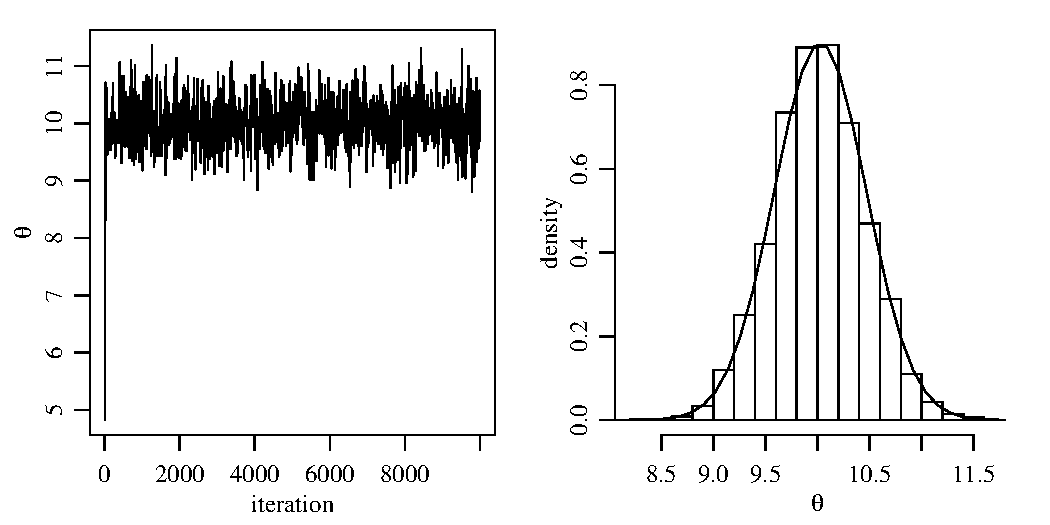
\includegraphics[scale=0.6]{metropolis_normal.pdf}
\caption{Results from the Metropolis sampler for the normal model.}
\label{met_norm}
\end{center}
\end{figure}


}

\frame{
\frametitle{Metropolis Hastings}

Let's recall what a Markov chain is.

\vskip 1em

%Recall that a Markov chain is a sequentially generated sequence $\{x^{(1)},,x^{(2)},\ldots\}$ such that the mechanism that generates $x^{(s+1)}$ can depend on the value of $x^{(s)}$ but not on anything that was in the sequence before it. A better way of putting this: for a Markov chain, the future depends on the present and not on the past. 

The Gibbs sampler and the Metropolis algorithm are both ways of generating Markov chains that approximate a target probability distribution. 

}

\frame{
Consider a simple example where our target probability distribution is 
$p_{o}(u,v),$ a bivariate distribution for two random variables $U$ and $V.$ 

\vskip 1em
In the one-sample normal problem, $U = \theta,$ $V = \sigma^2$ and 
$$p_{o}(u,v) = p(\theta, \sigma^2 | y).$$
\vskip 1em


\vskip 1em
\textcolor{blue}{Gibbs}: iteratively sample values of $U$ and $V$ from their conditional distributions. That is,
\begin{enumerate}
\item update $U:$ sample $u^{(s+1)} \sim p_{o}(u\mid v^{(s)})$
\item update $V:$ sample $v^{(s+1)} \sim p_{o}(v\mid u^{(s+1)}).$
\end{enumerate}
\vskip 1em
 \textcolor{blue}{Metropolis}: proposes changes to $X = (U,V)$ and then accepts or rejects those changes based on $p_o.$ 

}

\frame{


\vskip 1em
An alternative way to implement the Metropolis algorithm is to propose and then accept or reject change to one element at a time: 
\vskip 1em

\begin{enumerate}
\item update $U:$ 
\begin{enumerate}
\item sample $u^* \sim J_u(u\mid u^{(s)})$
\item compute $r = \dfrac{
p_o(u^*,v^{(s)})
}
{p_o(u^{(s)},v^{(s)})}
$
\item set $u^{(s+1)}$ equal to $u^*$ or $u^{(s+1)}$ with prob min(1,r) and 
max(0,1-r).
\end{enumerate}
\item update $V:$ sample $v^{(s+1)} \sim p_{o}(v\mid u^{(s+1)}).$
\begin{enumerate}
\item sample $v^* \sim J_u(v\mid v^{(s)})$
\item compute $r = \dfrac{
p_o(u^{(s+1)},v^*)
}
{p_o(u^{(s+1)},v^{(s)})}
$
\item set $v^{(s+1)}$ equal to $v^*$ or $v^{(s)}$ with prob min(1,r) and 
max(0,1-r).
\end{enumerate}
\end{enumerate}

Here, $J_u$ and $J_v$ are separate symmetric proposal distributions for $U$ and $V.$ 
}

\frame{
\begin{itemize}
\item The Metropolis algorithm generates proposals from $J_u$ and $J_v$
\item It accepts them with some probability min(1,r).
\item Similarly, each step of Gibbs can be seen as generating a proposal from a full conditional and then accepting it with probability 1. 
\item The Metropolis-Hastings (MH) algorithm generalizes both of these approaches by allowing arbitrary proposal distributions. 
\item The proposal distributions can be symmetric around the current values, full conditionals, or something else entirely. 
\end{itemize}
}

\frame{
A MH algorithm for approximating $p_o(u,v)$ runs as follows:
\begin{enumerate}
\item update $U:$ 
\begin{enumerate}
\item sample $u^* \sim J_u(u\mid u^{(s)},v^{(s)})$
\item compute $$r = \dfrac{
p_o(u^*,v^{(s)})
}
{p_o(u^{(s)},v^{(s)})}\times
\frac{
J_u(
u^{(s)} \mid u^*,v^{(s)}
)
}
{
J_u(
u^* \mid u^{(s)},v^{(s)}
)
}
$$
\item set $u^{(s+1)}$ equal to $u^*$ or $u^{(s+1)}$ with prob min(1,r) and 
max(0,1-r).
\end{enumerate}
\item update $V:$ 
\begin{enumerate}
\item sample $v^* \sim J_v(u\mid u^{(s+1)},v^{(s)})$
\item compute $$r = \dfrac{
p_o(u^{(s+1)},v^*)
}
{p_o(u^{(s+1)},v^{(s)})}\times
\frac{
J_u(
v^{(s+1)} \mid u^{(s+1)},v^{*)}
)
}
{
J_u(v^*
\mid u^{(s+1)},v^{(s)}
)
}
$$
\item set $v^{(s+1)}$ equal to $v^*$ or $v^{(s+1)}$ with prob min(1,r) and 
max(0,1-r).
\end{enumerate}
\end{enumerate}

Above: $J_u$ and $J_v$ are not required to be symmetric. They cannot depend on $U$ or $V$ values in our sequence previous to the most current values. This requirement ensures that the sequence is a Markov chain. 

}

\frame{

Doesn't the algorithm above look familiar? Yes, it looks a lot like Metropolis, except the acceptance ratio $r$ contains an extra factor:

\begin{itemize}
\item It contains the ratio of the prob of generating the \textcolor{red}{current value from the proposed} to the prob of generating the \textcolor{red}{proposed from the current.}
\item This can be viewed as a correction factor. 
\item If a value $u^*$ is much more likely to be proposed than the current value $u^{(s)}$ then we must \textcolor{red}{down-weight} the probability of accepting $u.$
\item Otherwise, such a value $u^*$ will be overrepresented in the chain.
\end{itemize}

Exercise 1: Show that Metropolis is a special case of MH. Hint: Think about the jumps J. 

Exercise 2: Show that Gibbs is a special case of MH. Hint: Show that r = 1.

}

\frame{
We implement the Metropolis algorithm for a Poisson regression model.
\begin{itemize}
\item We have a sample from a population of 52 song sparrows that was studied over the course of a summer and their reproductive activities were recorded.
\item In particular, their age and number of new offspring were recorded for each sparrow (Arcese et al., 1992). 
\item A simple probability model to fit the data would be a Poisson regression where, Y = number of  offspring conditional on x = age. 
\end{itemize}
Thus, we assume that $$Y|\theta_x \sim \text{Poisson}(\theta_x).$$ For stability of the model, we assume that the mean number of offspring $\theta_x$ is a smooth function of age. Thus, we express $\theta_x = \beta_1 + \beta_2x_ + \beta_3 x^2.$
}

\frame{
Remark: This parameterization allows some values of $\theta_x$ to be negative, so as an alternative we reparameterize and model the log-mean of Y, so that
$$\log E(Y|x) = \log \theta_x = \log(\beta_1 + \beta_2x_ + \beta_3 x^2)$$
which implies that $$\theta_x = \exp(\beta_1 + \beta_2x_ + \beta_3 x^2) = \exp(\bm{\beta}^T\bm{ x}).$$

Now back to the problem of implementing Metropolis. For this problem, we will write
$$\log E(Y_i|x_i) = \log(\beta_1 + \beta_2x_i + \beta_3 x_i^2) =\bm{ \beta}^T\bm{x_i} ,$$ where $x_i$ is the age of sparrow $i.$ We will abuse notation slightly and write $\bm{x_i} = (1, x_i, x_i^2).$
}

\frame{
\begin{itemize}
\item
We will assume the prior on the regression coefficients is iid Normal(0,100). 
\item Given a current value $ \bm{ \beta^{(s)}}$ and a value 
$ \bm{ \beta^*}$ generated from $J( \bm{ \beta^{*} },  \bm{ \beta^{(s)}})$
the acceptance ration for the Metropolis algorithm is:
\end{itemize}

$$
r = \frac{p( \bm{ \beta^{*}} | \bm{X}, \bm{y} )}
{
p( \bm{ \beta^{(s)}} | \bm{X}, \bm{y} )
}
= \frac{
\prod_{i=1}^n \text{dpois}(y_i, x_i^T  \beta^{*})
}
{\prod_{i=1}^n \text{dpois}(y_i, x_i^T  \beta^{(s)})
}
\times
\frac{
\prod_{j=1}^3 \text{dnorm}( \beta_j^{*},0,10)
}
{\prod_{j=1}^3 \text{dnorm}(  \beta_j^{(s)},0,10)
}.
$$
}

\frame{

\begin{itemize}
\item
We just need to specify the proposal distribution for $\theta^*$ 
\item A convenient choice is a multivariate normal distribution with mean $ \bm{ \beta^{(s)}}.$ 
\item In many problems, the posterior variance can be an efficient choice of a proposal variance. But we don't know it here. 
\item However, it's often sufficient to use a rough approximation. In a normal regression problem, the posterior variance will be close to $\sigma^2 (X^TX)^{-1}$ where $\sigma^2$ is the variance of $Y.$
\end{itemize}
In our problem: $ E \log Y = \beta^T x$ so we can try a proposal variance of $\hat{\sigma}^2(X^TX)^{-1}$ where $\hat{\sigma}^2$ is the sample variance of $\log(y +1/2).$

Remark: Note we add $1/2$ because otherwise $\log 0$ is undefined. The code of implementing the algorithm will be done in the corresponding lab.}

\frame{

\begin{figure}[htbp]
\begin{center}
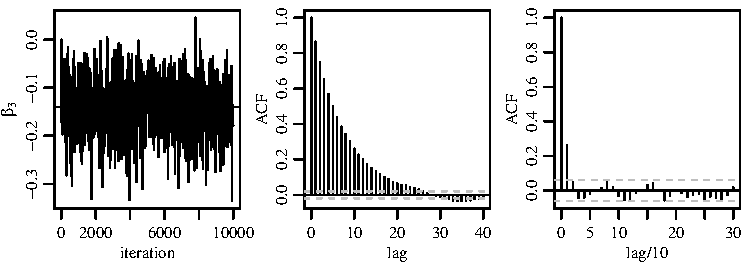
\includegraphics[width=0.8\textwidth]{metropolis_hastings/sparrow_plot1.pdf}
\caption{Plot of the Markov chain in $\beta_3$ along with autocorrelations functions}
\label{default}
\end{center}
\end{figure}

}

\frame{

More details of this example will be done in lab.


}


\end{document}